% !TeX program = pdflatex
% =============================================================================
% Fragenkatalog & Theorie-Notizen: Gewichtskraft & Federkraft
% UZH Praktikum I -- Sara Romer Urban, Kantonsschule im Lee, HS2026
% Klasse: 2e (26.08.2026)
%
% Kompiliertes PDF von gewichtskraft-federkraft-fragenkatalog.md -- enthaelt
% (A) die vollstaendigen Theorie-Notizen inkl. der Punkte, die im
% Arbeitsblatt selbst bewusst gekuerzt wurden, und (B) moegliche
% Impulsfragen pro Phase, analog zu kondensatoren-fragenkatalog.tex.
% Ausloeser: Feedback von Sara Romer -- Luftwiderstand-Vergleich und
% Astronauten-Waage-Mechanismus (Federpendel, den SuS noch nicht kennen)
% wurden aus dem Arbeitsblatt entfernt und stehen jetzt nur noch hier.
% =============================================================================
\documentclass[11pt,a4paper]{article}

\usepackage[T1]{fontenc}
\usepackage[utf8]{inputenc}
\usepackage[ngerman]{babel}
\usepackage{lmodern}
\usepackage[a4paper,margin=2.2cm,headheight=14pt]{geometry}
\usepackage{amsmath}
\usepackage{siunitx}
\sisetup{per-mode=fraction,fraction-command=\frac}
\usepackage{xcolor}
\usepackage{titlesec}
\usepackage{enumitem}
\usepackage{graphicx}
\usepackage{hyperref}

\setlength{\parindent}{0pt}
\setlength{\parskip}{0.5em}

\definecolor{titleblue}{HTML}{183A6B}
\definecolor{accentblue}{HTML}{2E6F9E}
\definecolor{darkgray}{HTML}{4A4A4A}

\hypersetup{
  colorlinks=true,
  urlcolor=accentblue,
  linkcolor=accentblue,
  pdftitle={Fragenkatalog: Gewichtskraft \& Federkraft},
  pdfauthor={Loris Keller}
}

\titleformat{\section}{\Large\bfseries\color{titleblue}}{\thesection}{0.6em}{}
\titleformat{\subsection}{\large\bfseries\color{accentblue}}{}{0em}{}
\titlespacing*{\section}{0pt}{1.1em}{0.5em}
\titlespacing*{\subsection}{0pt}{0.9em}{0.3em}

\newcommand{\Frage}[1]{\textbf{Frage:} #1\par}
\newcommand{\Antwort}[1]{\textbf{Antwort:} #1\par}
\newcommand{\Erklaerung}[1]{\textit{Erklärung:} #1}
\newcommand{\FrageBlock}[3]{\Frage{#1}\Antwort{#2}\Erklaerung{#3}\vspace{0.6em}}

\pagestyle{plain}

\begin{document}

{\Large\bfseries\color{titleblue} Fragenkatalog \& Theorie-Notizen --- Gewichtskraft \& Federkraft}\\[0.2em]
{\large\color{accentblue} Vorbereitung für die Lehrperson}\\[0.4em]
\textcolor{darkgray}{Klasse: 2e, 26.08.2026.}

\vspace{0.3em}
{\noindent\color{accentblue}\rule{\linewidth}{0.8pt}}
\vspace{0.5em}

Lehrpersonen-Vorbereitung zur Doppellektion. Teil A enthält die
vollständigen Theorie-Notizen inklusive der Punkte, die im ausgeteilten
Arbeitsblatt bewusst gekürzt wurden (das Arbeitsblatt bleibt minimalistisch,
diese Notizen hier nicht). Teil B enthält mögliche Impulsfragen pro Phase,
analog zu \texttt{kondensatoren-\allowbreak fragenkatalog.md}/\texttt{.tex}.

Auslöser: Feedback von Sara Romer nach Durchsicht des ersten Entwurfs. Zeit
könnte knapp werden (2e ist bezüglich Diskussionsbeteiligung schwer
einzuschätzen), und der Mechanismus der Astronauten-Trägheitswaage ist für
die SuS unklar, da sie das Federpendel noch nicht kennen. Das
Hammer-und-Feder-Beispiel (Apollo~15) wurde daraufhin zunächst nur beim
Luftwiderstand-Vergleich gekürzt, anschliessend aber ganz aus dem
Arbeitsblatt entfernt: Luftwiderstand spielt bei diesem Effekt eine Rolle
und gehört nicht zum Thema dieser Doppellektion.

\section*{Teil A --- Theorie-Notizen für die Lektion}

\subsection*{Gewichtskraft (Theorie 1)}

\begin{itemize}[leftmargin=1.2cm,itemsep=0.3em]
  \item Masse $m$ = Trägheit eines Körpers, ortsunabhängig, ändert sich nie.
  \item Gewichtskraft $F_G=m\cdot g$ (Einheit N): die Kraft, mit der ein
  Himmelskörper eine Masse anzieht.
  \item Ortsfaktor $g$: Erde $\SI{9.81}{\meter\per\second\squared}$, Mond
  $\SI{1.62}{\meter\per\second\squared}$, Faktor rund 6 zwischen den beiden.
\end{itemize}

\subsection*{Federkraft-Konzept (Theorie 2)}

\begin{itemize}[leftmargin=1.2cm,itemsep=0.3em]
  \item Kräftegleichgewicht: Die Feder dehnt sich, bis $F=F_G$ gilt; die
  Dehnung an diesem Punkt zeigt die Kraft an.
  \item Längenänderung $\Delta x$ (nicht die absolute Federlänge $x$) ist
  massgebend, besonders bei einer bereits vorgespannten Feder.
  \item Kalibrierung: bekannte Gewichtskräfte (z.\,B.
  100-g-Schokoladentafeln, je rund 1 N) an eine unbeschriftete Feder
  hängen, Dehnung markieren, daraus entsteht eine Newton-Skala.
  \item \textbf{Vollständiges Rechenbeispiel}, im Arbeitsblatt nur noch als
  ein Satz ohne Rechnung: $F_G=\SI{0.1}{\kilogram}\cdot\SI{9.81}{\meter\per\second\squared}\approx\SI{1}{\newton}$
  für eine 100-g-Tafel. Bei Bedarf im Plenum vorrechnen.
  \item $F=D\cdot\Delta x$ (Hookesches Gesetz) und die Federkonstante $D$
  selbst werden bewusst \textbf{nicht} im Arbeitsblatt vorweggenommen: Die
  SuS leiten beides im Aufgabenblatt aus eigenen Messdaten her. Auch die
  Lernziele-Box ist deshalb absichtlich kompetenzorientiert statt
  ergebnisoffen formuliert.
\end{itemize}

\subsection*{Bewusst aus dem Arbeitsblatt entfernte Inhalte}

Diese beiden Themen sind vollständig aus dem Arbeitsblatt gestrichen, nicht
nur gekürzt. Beide können bei Interesse rein mündlich erwähnt werden, sind
aber kein Bestandteil der Lektion mehr.

\begin{enumerate}[leftmargin=1.2cm,itemsep=0.4em]
  \item \textbf{Hammer-und-Feder-Beispiel auf dem Mond} (Apollo~15,
  Commander David Scott, 1971). Ursprünglich als Beispiel dafür gedacht,
  dass die Fallbeschleunigung $a=g$ unabhängig von der Masse ist (aus
  $F=m\cdot a$ und $F_G=m\cdot a=m\cdot g$): Die grössere Gewichtskraft
  eines Hammers wird durch seine ebenfalls grössere Trägheit exakt
  kompensiert, deshalb fallen Hammer und Feder auf dem Mond gleichzeitig.
  Vollständig gestrichen, weil der Effekt nur unter Ausschluss von
  Luftwiderstand korrekt erklärbar ist, ein Konzept, das nicht zum Thema
  dieser Doppellektion gehört (auf der Erde bremst der Luftwiderstand die
  leichte, grossflächige Feder viel stärker als den kompakten Hammer).
  \item \textbf{Astronauten-Trägheitswaage (Federpendel-Mechanismus).} Auf
  der ISS lässt ein Gerät die Astronaut:innen auf einem federnden Sitz
  kurz hin- und herschwingen; je grösser die Masse, desto langsamer
  schwingt das System, und aus der Schwingungsdauer lässt sich die Masse
  bestimmen, ganz ohne Gewichtskraft. Die SuS kennen das Federpendel noch
  nicht (Thema erst in einer späteren Schwingungs-Einheit), deshalb wurde
  auch die einfache Version der Teilfrage (nur \glqq Trägheit\grqq{} als
  erwartete Antwort, ohne Mechanismus) ganz aus dem Arbeitsblatt entfernt.
  Den Mechanismus nur mündlich erwähnen, wenn eine neugierige Frage kommt.
  Keine Herleitung verlangen.
  \begin{center}
    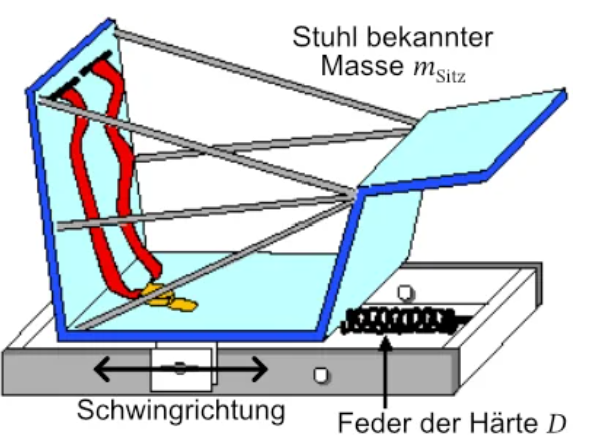
\includegraphics[width=5cm]{Bilder/astronauten_waage.png}
  \end{center}
  {\scriptsize Prinzipskizze: Ein Sitz bekannter Masse $m_{\text{Sitz}}$
  schwingt auf einer Feder der Härte $D$; aus der Schwingungsdauer lässt
  sich die Gesamtmasse (Sitz plus Astronaut:in) bestimmen.}
\end{enumerate}

\subsection*{Hinweis zur Zeitplanung}

Sara Romer weist darauf hin, dass die Zeit knapp werden kann, da bei
Klasse 2e nie sicher ist, wie viel die SuS mitreden werden. Die
Verlaufsplanung (\texttt{gewichtskraft-\allowbreak federkraft-\allowbreak
verlaufsplanung.\allowbreak tex}) enthält bereits eine Kürzungsreihenfolge
(zuerst Ausblick, danach Einheitenumrechnung, nie die Lernaufgabe). Die
beiden oben entfernten Punkte sind jetzt ohnehin kürzer als zuvor. Das
entlastet den Zeitplan zusätzlich, unabhängig von der
Diskussionsbeteiligung der Klasse.

\section*{Teil B --- Fragenkatalog (Impulsfragen pro Phase)}

\subsection*{Wiederholung}

\FrageBlock{Was bedeutet es, wenn ein Wagen bei gleicher Kraft schneller beschleunigt als ein anderer?}
{Der schnellere Wagen hat eine kleinere Masse (weniger Trägheit).}
{Knüpft an $F\sim a$ aus der letzten Stunde an und bereitet den Trägheitsbegriff für die heutige Lektion vor.}

\subsection*{Übung: Fussballschuss}

\FrageBlock{Warum tut ein harter Schuss mit blossem Fuss mehr weh als ein sanfter?}
{Weil die Kraft, die Fuss und Ball gegenseitig aufeinander ausüben, bei kürzerer Kontaktzeit und grösserer Geschwindigkeitsänderung viel grösser ist.}
{Reine Anwendung von $F=m\cdot a$, motiviert die anschliessende Rechnung mit konkreten Zahlen.}

\subsection*{Aktivierung 1: Steinstoss}

\FrageBlock{Würde es auf einem noch kleineren Himmelskörper als dem Mond (z.\,B. einem Asteroiden) auch gleich weh tun?}
{Ja, genauso, solange derselbe Stein mit derselben Aufprallgeschwindigkeit verwendet wird.}
{Verstärkt, dass die Trägheit unabhängig vom Ort ist. Der Ortsfaktor spielt für den Aufprallschmerz keine Rolle.}

\subsection*{Aktivierung 2: Golfball auf dem Mond}

\FrageBlock{Was würde passieren, wenn der Golfball auf einem Planeten mit noch grösserem Ortsfaktor als die Erde geschlagen würde?}
{Er würde weniger weit fliegen als auf der Erde.}
{Testet das Verständnis der Gewichtskraft-Ortsfaktor-Beziehung in die entgegengesetzte Richtung zum eigentlichen Beispiel.}

\subsection*{Theorie 1: Gewichtskraft}

\FrageBlock{Wenn ich auf der Erde 700 N wiege, wie viel wiege ich ungefähr auf dem Mond, ohne zu rechnen?}
{Ungefähr ein Sechstel, also rund 116 N.}
{Kopfrechnen zur Verinnerlichung des Faktors 6, bevor die Astronautin-Aufgabe die exakte Rechnung verlangt.}

\subsection*{Theorie 2: Federkraft-Konzept}

\FrageBlock{Warum zeigt eine Feder ohne angehängte Masse eigentlich \glqq 0 N\grqq{} und nicht irgendeinen anderen Wert?}
{Weil der Nullpunkt beim Kalibrieren extra auf die ungespannte (oder bereits leicht vorgespannte) Lage gesetzt wird.}
{Verstärkt die $\Delta x$-vs-$x$-Unterscheidung aus der Hinweisbox.}

\subsection*{Übung: Wiegen im Weltraum}

\FrageBlock{Wie messen Astronaut:innen ihre Masse wirklich, wenn ein Federkraftmesser nicht funktioniert?}
{Über die Trägheit: Ein Gerät lässt sie auf einem federnden Sitz kurz hin- und herschwingen; je grösser die Masse, desto langsamer schwingt das System, und aus der Schwingungsdauer lässt sich die Masse berechnen.}
{Diese Erklärung wurde aus dem Arbeitsblatt entfernt, da die SuS das Federpendel und Schwingungen allgemein noch nicht kennen (Feedback von Sara Romer). Nur mündlich erwähnen, die ausführliche Herleitung folgt erst in der späteren Schwingungs-Einheit.}

\subsection*{Übung: Einheitenumrechnung}

\FrageBlock{Warum wird die Federkonstante im Laden oft in N/cm angegeben statt in der SI-Einheit N/m?}
{Weil die typischen Auslenkungen einer Feder im Alltag eher im Zentimeterbereich liegen und die Zahlenwerte in N/cm dadurch handlicher sind.}
{Verbindet die Alltagspraxis mit der SI-Konvention, die die SuS in der Aufgabe anwenden müssen.}

\end{document}
